\documentclass[tikz,border=10pt]{standalone}
\begin{document}
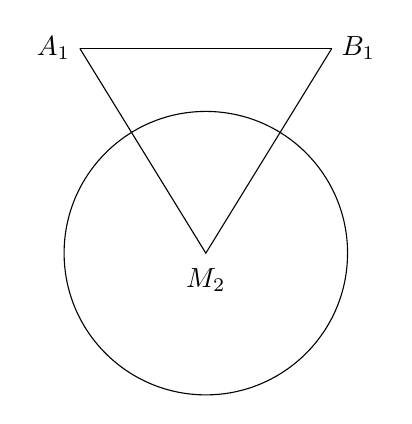
\begin{tikzpicture}
  \coordinate (M2) at (0,0);
  \coordinate (A1) at (-1.6,2.6);
  \coordinate (B1) at (1.6,2.6);
  \draw (M2) circle (1.8);
  \draw (A1) -- (M2) -- (B1);
  \draw (A1) -- (B1);
  \node[left] at (A1) {$A_1$};
  \node[right] at (B1) {$B_1$};
  \node[below=2pt] at (M2) {$M_2$};
\end{tikzpicture}
\end{document}
